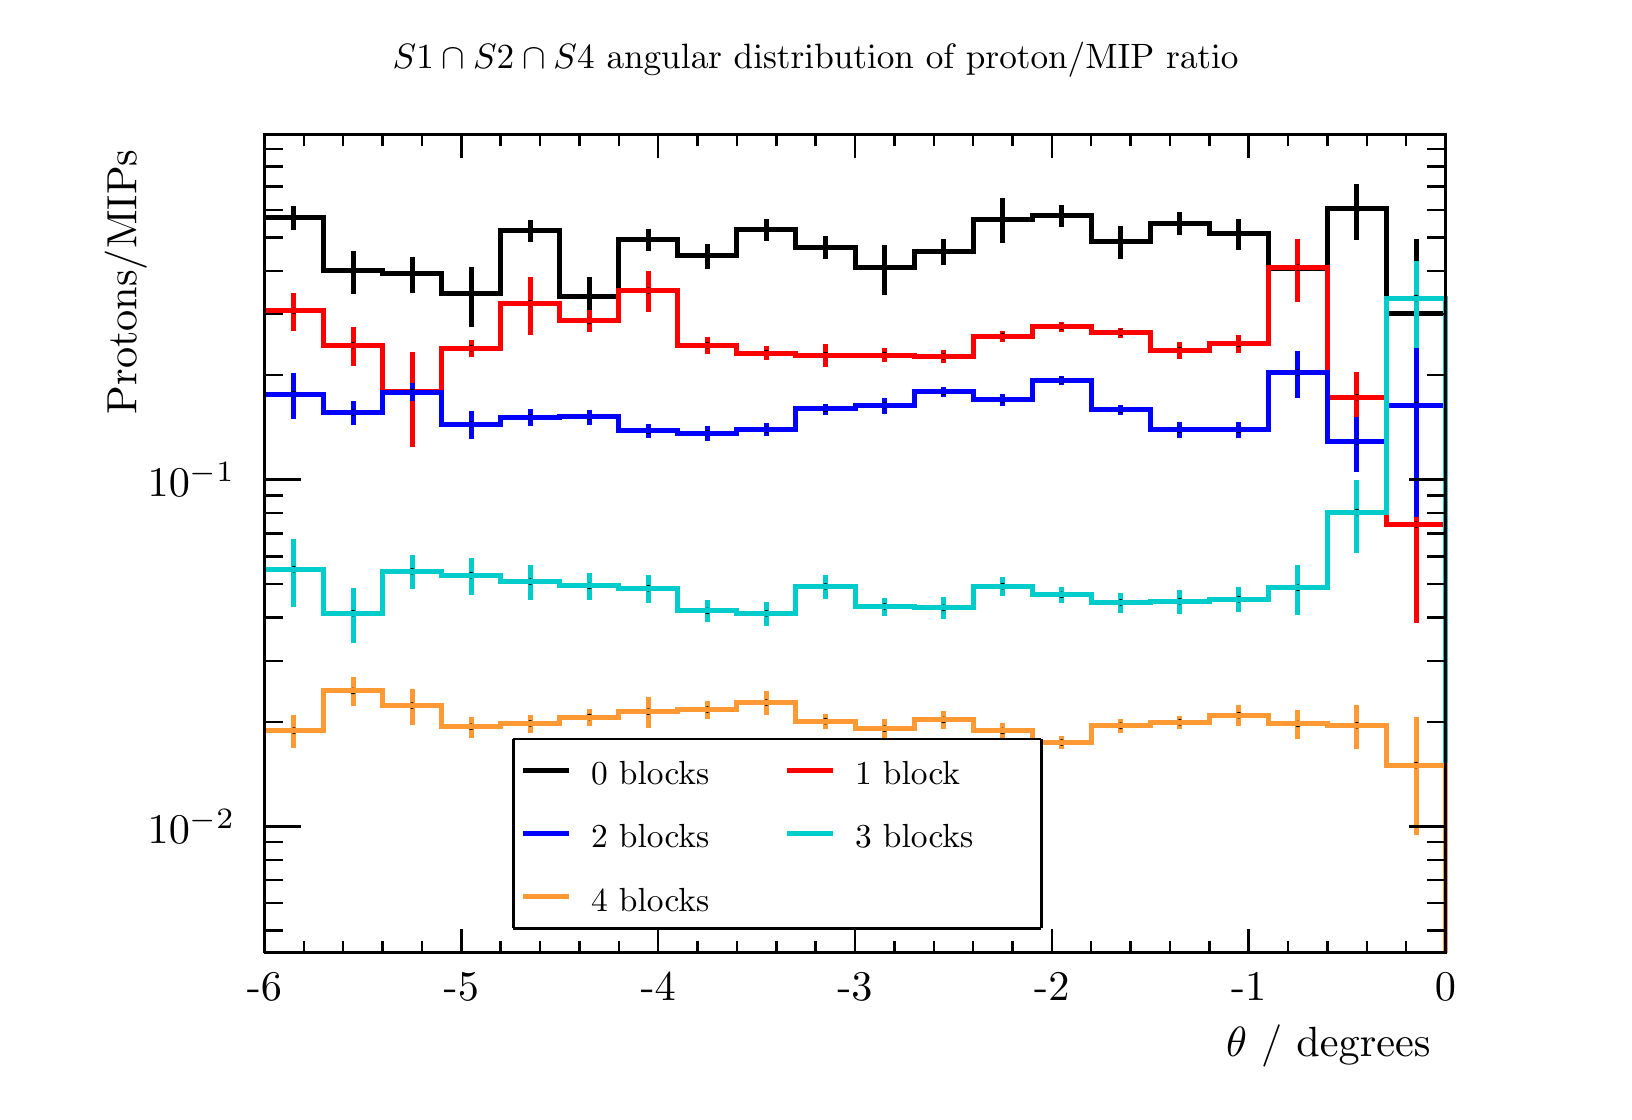
\begin{tikzpicture}
\pgfdeclareplotmark{cross} {
\pgfpathmoveto{\pgfpoint{-0.3\pgfplotmarksize}{\pgfplotmarksize}}
\pgfpathlineto{\pgfpoint{+0.3\pgfplotmarksize}{\pgfplotmarksize}}
\pgfpathlineto{\pgfpoint{+0.3\pgfplotmarksize}{0.3\pgfplotmarksize}}
\pgfpathlineto{\pgfpoint{+1\pgfplotmarksize}{0.3\pgfplotmarksize}}
\pgfpathlineto{\pgfpoint{+1\pgfplotmarksize}{-0.3\pgfplotmarksize}}
\pgfpathlineto{\pgfpoint{+0.3\pgfplotmarksize}{-0.3\pgfplotmarksize}}
\pgfpathlineto{\pgfpoint{+0.3\pgfplotmarksize}{-1.\pgfplotmarksize}}
\pgfpathlineto{\pgfpoint{-0.3\pgfplotmarksize}{-1.\pgfplotmarksize}}
\pgfpathlineto{\pgfpoint{-0.3\pgfplotmarksize}{-0.3\pgfplotmarksize}}
\pgfpathlineto{\pgfpoint{-1.\pgfplotmarksize}{-0.3\pgfplotmarksize}}
\pgfpathlineto{\pgfpoint{-1.\pgfplotmarksize}{0.3\pgfplotmarksize}}
\pgfpathlineto{\pgfpoint{-0.3\pgfplotmarksize}{0.3\pgfplotmarksize}}
\pgfpathclose
\pgfusepathqstroke
}
\pgfdeclareplotmark{cross*} {
\pgfpathmoveto{\pgfpoint{-0.3\pgfplotmarksize}{\pgfplotmarksize}}
\pgfpathlineto{\pgfpoint{+0.3\pgfplotmarksize}{\pgfplotmarksize}}
\pgfpathlineto{\pgfpoint{+0.3\pgfplotmarksize}{0.3\pgfplotmarksize}}
\pgfpathlineto{\pgfpoint{+1\pgfplotmarksize}{0.3\pgfplotmarksize}}
\pgfpathlineto{\pgfpoint{+1\pgfplotmarksize}{-0.3\pgfplotmarksize}}
\pgfpathlineto{\pgfpoint{+0.3\pgfplotmarksize}{-0.3\pgfplotmarksize}}
\pgfpathlineto{\pgfpoint{+0.3\pgfplotmarksize}{-1.\pgfplotmarksize}}
\pgfpathlineto{\pgfpoint{-0.3\pgfplotmarksize}{-1.\pgfplotmarksize}}
\pgfpathlineto{\pgfpoint{-0.3\pgfplotmarksize}{-0.3\pgfplotmarksize}}
\pgfpathlineto{\pgfpoint{-1.\pgfplotmarksize}{-0.3\pgfplotmarksize}}
\pgfpathlineto{\pgfpoint{-1.\pgfplotmarksize}{0.3\pgfplotmarksize}}
\pgfpathlineto{\pgfpoint{-0.3\pgfplotmarksize}{0.3\pgfplotmarksize}}
\pgfpathclose
\pgfusepathqfillstroke
}
\pgfdeclareplotmark{newstar} {
\pgfpathmoveto{\pgfqpoint{0pt}{\pgfplotmarksize}}
\pgfpathlineto{\pgfqpointpolar{44}{0.5\pgfplotmarksize}}
\pgfpathlineto{\pgfqpointpolar{18}{\pgfplotmarksize}}
\pgfpathlineto{\pgfqpointpolar{-20}{0.5\pgfplotmarksize}}
\pgfpathlineto{\pgfqpointpolar{-54}{\pgfplotmarksize}}
\pgfpathlineto{\pgfqpointpolar{-90}{0.5\pgfplotmarksize}}
\pgfpathlineto{\pgfqpointpolar{234}{\pgfplotmarksize}}
\pgfpathlineto{\pgfqpointpolar{198}{0.5\pgfplotmarksize}}
\pgfpathlineto{\pgfqpointpolar{162}{\pgfplotmarksize}}
\pgfpathlineto{\pgfqpointpolar{134}{0.5\pgfplotmarksize}}
\pgfpathclose
\pgfusepathqstroke
}
\pgfdeclareplotmark{newstar*} {
\pgfpathmoveto{\pgfqpoint{0pt}{\pgfplotmarksize}}
\pgfpathlineto{\pgfqpointpolar{44}{0.5\pgfplotmarksize}}
\pgfpathlineto{\pgfqpointpolar{18}{\pgfplotmarksize}}
\pgfpathlineto{\pgfqpointpolar{-20}{0.5\pgfplotmarksize}}
\pgfpathlineto{\pgfqpointpolar{-54}{\pgfplotmarksize}}
\pgfpathlineto{\pgfqpointpolar{-90}{0.5\pgfplotmarksize}}
\pgfpathlineto{\pgfqpointpolar{234}{\pgfplotmarksize}}
\pgfpathlineto{\pgfqpointpolar{198}{0.5\pgfplotmarksize}}
\pgfpathlineto{\pgfqpointpolar{162}{\pgfplotmarksize}}
\pgfpathlineto{\pgfqpointpolar{134}{0.5\pgfplotmarksize}}
\pgfpathclose
\pgfusepathqfillstroke
}
\definecolor{c}{rgb}{1,1,1};
\draw [color=c, fill=c] (0,0) rectangle (20,13.4957);
\draw [color=c, fill=c] (3,1.75444) rectangle (18,12.1461);
\definecolor{c}{rgb}{0,0,0};
\draw [c,line width=0.9] (3,1.75444) -- (3,12.1461) -- (18,12.1461) -- (18,1.75444) -- (3,1.75444);
\definecolor{c}{rgb}{1,1,1};
\draw [color=c, fill=c] (3,1.75444) rectangle (18,12.1461);
\definecolor{c}{rgb}{0,0,0};
\draw [c,line width=0.9] (3,1.75444) -- (3,12.1461) -- (18,12.1461) -- (18,1.75444) -- (3,1.75444);
\draw [c,line width=0.9] (3,1.75444) -- (3.75,1.75444) -- (3.75,1.75444) -- (4.5,1.75444) -- (4.5,1.75444) -- (5.25,1.75444) -- (5.25,1.75444) -- (6,1.75444) -- (6,1.75444) -- (6.75,1.75444) -- (6.75,1.75444) -- (7.5,1.75444) -- (7.5,1.75444) --
 (8.25,1.75444) -- (8.25,1.75444) -- (9,1.75444) -- (9,1.75444) -- (9.75,1.75444) -- (9.75,1.75444) -- (10.5,1.75444) -- (10.5,1.75444) -- (11.25,1.75444) -- (11.25,1.75444) -- (12,1.75444) -- (12,1.75444) -- (12.75,1.75444) -- (12.75,1.75444) --
 (13.5,1.75444) -- (13.5,1.75444) -- (14.25,1.75444) -- (14.25,1.75444) -- (15,1.75444) -- (15,1.75444) -- (15.75,1.75444) -- (15.75,1.75444) -- (16.5,1.75444) -- (16.5,1.75444) -- (17.25,1.75444) -- (17.25,1.75444) -- (18,1.75444) -- (18,1.75444);
\draw [c,line width=0.9] (3,1.75444) -- (18,1.75444);
\draw [c,line width=0.9] (3,2.05809) -- (3,1.75444);
\draw [c,line width=0.9] (3.5,1.90627) -- (3.5,1.75444);
\draw [c,line width=0.9] (4,1.90627) -- (4,1.75444);
\draw [c,line width=0.9] (4.5,1.90627) -- (4.5,1.75444);
\draw [c,line width=0.9] (5,1.90627) -- (5,1.75444);
\draw [c,line width=0.9] (5.5,2.05809) -- (5.5,1.75444);
\draw [c,line width=0.9] (6,1.90627) -- (6,1.75444);
\draw [c,line width=0.9] (6.5,1.90627) -- (6.5,1.75444);
\draw [c,line width=0.9] (7,1.90627) -- (7,1.75444);
\draw [c,line width=0.9] (7.5,1.90627) -- (7.5,1.75444);
\draw [c,line width=0.9] (8,2.05809) -- (8,1.75444);
\draw [c,line width=0.9] (8.5,1.90627) -- (8.5,1.75444);
\draw [c,line width=0.9] (9,1.90627) -- (9,1.75444);
\draw [c,line width=0.9] (9.5,1.90627) -- (9.5,1.75444);
\draw [c,line width=0.9] (10,1.90627) -- (10,1.75444);
\draw [c,line width=0.9] (10.5,2.05809) -- (10.5,1.75444);
\draw [c,line width=0.9] (11,1.90627) -- (11,1.75444);
\draw [c,line width=0.9] (11.5,1.90627) -- (11.5,1.75444);
\draw [c,line width=0.9] (12,1.90627) -- (12,1.75444);
\draw [c,line width=0.9] (12.5,1.90627) -- (12.5,1.75444);
\draw [c,line width=0.9] (13,2.05809) -- (13,1.75444);
\draw [c,line width=0.9] (13.5,1.90627) -- (13.5,1.75444);
\draw [c,line width=0.9] (14,1.90627) -- (14,1.75444);
\draw [c,line width=0.9] (14.5,1.90627) -- (14.5,1.75444);
\draw [c,line width=0.9] (15,1.90627) -- (15,1.75444);
\draw [c,line width=0.9] (15.5,2.05809) -- (15.5,1.75444);
\draw [c,line width=0.9] (16,1.90627) -- (16,1.75444);
\draw [c,line width=0.9] (16.5,1.90627) -- (16.5,1.75444);
\draw [c,line width=0.9] (17,1.90627) -- (17,1.75444);
\draw [c,line width=0.9] (17.5,1.90627) -- (17.5,1.75444);
\draw [c,line width=0.9] (18,2.05809) -- (18,1.75444);
\draw [anchor=base] (3,1.14713) node[scale=1.52731, color=c, rotate=0]{-6};
\draw [anchor=base] (5.5,1.14713) node[scale=1.52731, color=c, rotate=0]{-5};
\draw [anchor=base] (8,1.14713) node[scale=1.52731, color=c, rotate=0]{-4};
\draw [anchor=base] (10.5,1.14713) node[scale=1.52731, color=c, rotate=0]{-3};
\draw [anchor=base] (13,1.14713) node[scale=1.52731, color=c, rotate=0]{-2};
\draw [anchor=base] (15.5,1.14713) node[scale=1.52731, color=c, rotate=0]{-1};
\draw [anchor=base] (18,1.14713) node[scale=1.52731, color=c, rotate=0]{0};
\draw [anchor= east] (18,0.566819) node[scale=1.52731, color=c, rotate=0]{$\theta$ / degrees};
\draw [c,line width=0.9] (3,12.1461) -- (18,12.1461);
\draw [c,line width=0.9] (3,11.8425) -- (3,12.1461);
\draw [c,line width=0.9] (3.5,11.9943) -- (3.5,12.1461);
\draw [c,line width=0.9] (4,11.9943) -- (4,12.1461);
\draw [c,line width=0.9] (4.5,11.9943) -- (4.5,12.1461);
\draw [c,line width=0.9] (5,11.9943) -- (5,12.1461);
\draw [c,line width=0.9] (5.5,11.8425) -- (5.5,12.1461);
\draw [c,line width=0.9] (6,11.9943) -- (6,12.1461);
\draw [c,line width=0.9] (6.5,11.9943) -- (6.5,12.1461);
\draw [c,line width=0.9] (7,11.9943) -- (7,12.1461);
\draw [c,line width=0.9] (7.5,11.9943) -- (7.5,12.1461);
\draw [c,line width=0.9] (8,11.8425) -- (8,12.1461);
\draw [c,line width=0.9] (8.5,11.9943) -- (8.5,12.1461);
\draw [c,line width=0.9] (9,11.9943) -- (9,12.1461);
\draw [c,line width=0.9] (9.5,11.9943) -- (9.5,12.1461);
\draw [c,line width=0.9] (10,11.9943) -- (10,12.1461);
\draw [c,line width=0.9] (10.5,11.8425) -- (10.5,12.1461);
\draw [c,line width=0.9] (11,11.9943) -- (11,12.1461);
\draw [c,line width=0.9] (11.5,11.9943) -- (11.5,12.1461);
\draw [c,line width=0.9] (12,11.9943) -- (12,12.1461);
\draw [c,line width=0.9] (12.5,11.9943) -- (12.5,12.1461);
\draw [c,line width=0.9] (13,11.8425) -- (13,12.1461);
\draw [c,line width=0.9] (13.5,11.9943) -- (13.5,12.1461);
\draw [c,line width=0.9] (14,11.9943) -- (14,12.1461);
\draw [c,line width=0.9] (14.5,11.9943) -- (14.5,12.1461);
\draw [c,line width=0.9] (15,11.9943) -- (15,12.1461);
\draw [c,line width=0.9] (15.5,11.8425) -- (15.5,12.1461);
\draw [c,line width=0.9] (16,11.9943) -- (16,12.1461);
\draw [c,line width=0.9] (16.5,11.9943) -- (16.5,12.1461);
\draw [c,line width=0.9] (17,11.9943) -- (17,12.1461);
\draw [c,line width=0.9] (17.5,11.9943) -- (17.5,12.1461);
\draw [c,line width=0.9] (18,11.8425) -- (18,12.1461);
\draw [c,line width=0.9] (3,1.75444) -- (3,12.1461);
\draw [c,line width=0.9] (3.231,2.0349) -- (3,2.0349);
\draw [c,line width=0.9] (3.231,2.38353) -- (3,2.38353);
\draw [c,line width=0.9] (3.231,2.67829) -- (3,2.67829);
\draw [c,line width=0.9] (3.231,2.93362) -- (3,2.93362);
\draw [c,line width=0.9] (3.231,3.15883) -- (3,3.15883);
\draw [c,line width=0.9] (3.462,3.3603) -- (3,3.3603);
\draw [anchor= east] (2.82,3.3603) node[scale=1.52731, color=c, rotate=0]{$10^{-2}$};
\draw [c,line width=0.9] (3.231,4.68569) -- (3,4.68569);
\draw [c,line width=0.9] (3.231,5.46099) -- (3,5.46099);
\draw [c,line width=0.9] (3.231,6.01108) -- (3,6.01108);
\draw [c,line width=0.9] (3.231,6.43776) -- (3,6.43776);
\draw [c,line width=0.9] (3.231,6.78639) -- (3,6.78639);
\draw [c,line width=0.9] (3.231,7.08114) -- (3,7.08114);
\draw [c,line width=0.9] (3.231,7.33647) -- (3,7.33647);
\draw [c,line width=0.9] (3.231,7.56169) -- (3,7.56169);
\draw [c,line width=0.9] (3.462,7.76315) -- (3,7.76315);
\draw [anchor= east] (2.82,7.76315) node[scale=1.52731, color=c, rotate=0]{$10^{-1}$};
\draw [c,line width=0.9] (3.231,9.08854) -- (3,9.08854);
\draw [c,line width=0.9] (3.231,9.86385) -- (3,9.86385);
\draw [c,line width=0.9] (3.231,10.4139) -- (3,10.4139);
\draw [c,line width=0.9] (3.231,10.8406) -- (3,10.8406);
\draw [c,line width=0.9] (3.231,11.1892) -- (3,11.1892);
\draw [c,line width=0.9] (3.231,11.484) -- (3,11.484);
\draw [c,line width=0.9] (3.231,11.7393) -- (3,11.7393);
\draw [c,line width=0.9] (3.231,11.9645) -- (3,11.9645);
\draw [anchor= east] (1.24,12.1461) node[scale=1.52731, color=c, rotate=90]{ Protons/MIPs};
\draw [c,line width=0.9] (18,1.75444) -- (18,12.1461);
\draw [c,line width=0.9] (17.769,2.0349) -- (18,2.0349);
\draw [c,line width=0.9] (17.769,2.38353) -- (18,2.38353);
\draw [c,line width=0.9] (17.769,2.67829) -- (18,2.67829);
\draw [c,line width=0.9] (17.769,2.93362) -- (18,2.93362);
\draw [c,line width=0.9] (17.769,3.15883) -- (18,3.15883);
\draw [c,line width=0.9] (17.538,3.3603) -- (18,3.3603);
\draw [c,line width=0.9] (17.769,4.68569) -- (18,4.68569);
\draw [c,line width=0.9] (17.769,5.46099) -- (18,5.46099);
\draw [c,line width=0.9] (17.769,6.01108) -- (18,6.01108);
\draw [c,line width=0.9] (17.769,6.43776) -- (18,6.43776);
\draw [c,line width=0.9] (17.769,6.78639) -- (18,6.78639);
\draw [c,line width=0.9] (17.769,7.08114) -- (18,7.08114);
\draw [c,line width=0.9] (17.769,7.33647) -- (18,7.33647);
\draw [c,line width=0.9] (17.769,7.56169) -- (18,7.56169);
\draw [c,line width=0.9] (17.538,7.76315) -- (18,7.76315);
\draw [c,line width=0.9] (17.769,9.08854) -- (18,9.08854);
\draw [c,line width=0.9] (17.769,9.86385) -- (18,9.86385);
\draw [c,line width=0.9] (17.769,10.4139) -- (18,10.4139);
\draw [c,line width=0.9] (17.769,10.8406) -- (18,10.8406);
\draw [c,line width=0.9] (17.769,11.1892) -- (18,11.1892);
\draw [c,line width=0.9] (17.769,11.484) -- (18,11.484);
\draw [c,line width=0.9] (17.769,11.7393) -- (18,11.7393);
\draw [c,line width=0.9] (17.769,11.9645) -- (18,11.9645);
\draw [c,line width=1.8] (3.375,10.9293) -- (3.375,11.0925);
\draw [c,line width=1.8] (3.375,11.0925) -- (3.375,11.2429);
\foreach \P in {(3.375,11.0925)}{\draw[mark options={color=c,fill=c},mark size=2.402402pt,mark=*,mark size=1pt] plot coordinates {\P};}
\draw [c,line width=1.8] (4.125,10.1235) -- (4.125,10.4149);
\draw [c,line width=1.8] (4.125,10.4149) -- (4.125,10.6676);
\foreach \P in {(4.125,10.4149)}{\draw[mark options={color=c,fill=c},mark size=2.402402pt,mark=*,mark size=1pt] plot coordinates {\P};}
\draw [c,line width=1.8] (4.875,10.1301) -- (4.875,10.3756);
\draw [c,line width=1.8] (4.875,10.3756) -- (4.875,10.5931);
\foreach \P in {(4.875,10.3756)}{\draw[mark options={color=c,fill=c},mark size=2.402402pt,mark=*,mark size=1pt] plot coordinates {\P};}
\draw [c,line width=1.8] (5.625,9.69711) -- (5.625,10.1214);
\draw [c,line width=1.8] (5.625,10.1214) -- (5.625,10.4684);
\foreach \P in {(5.625,10.1214)}{\draw[mark options={color=c,fill=c},mark size=2.402402pt,mark=*,mark size=1pt] plot coordinates {\P};}
\draw [c,line width=1.8] (6.375,10.7848) -- (6.375,10.93);
\draw [c,line width=1.8] (6.375,10.93) -- (6.375,11.065);
\foreach \P in {(6.375,10.93)}{\draw[mark options={color=c,fill=c},mark size=2.402402pt,mark=*,mark size=1pt] plot coordinates {\P};}
\draw [c,line width=1.8] (7.125,9.79375) -- (7.125,10.0863);
\draw [c,line width=1.8] (7.125,10.0863) -- (7.125,10.34);
\foreach \P in {(7.125,10.0863)}{\draw[mark options={color=c,fill=c},mark size=2.402402pt,mark=*,mark size=1pt] plot coordinates {\P};}
\draw [c,line width=1.8] (7.875,10.6639) -- (7.875,10.8086);
\draw [c,line width=1.8] (7.875,10.8086) -- (7.875,10.9431);
\foreach \P in {(7.875,10.8086)}{\draw[mark options={color=c,fill=c},mark size=2.402402pt,mark=*,mark size=1pt] plot coordinates {\P};}
\draw [c,line width=1.8] (8.625,10.4345) -- (8.625,10.6048);
\draw [c,line width=1.8] (8.625,10.6048) -- (8.625,10.7612);
\foreach \P in {(8.625,10.6048)}{\draw[mark options={color=c,fill=c},mark size=2.402402pt,mark=*,mark size=1pt] plot coordinates {\P};}
\draw [c,line width=1.8] (9.375,10.7953) -- (9.375,10.9398);
\draw [c,line width=1.8] (9.375,10.9398) -- (9.375,11.0741);
\foreach \P in {(9.375,10.9398)}{\draw[mark options={color=c,fill=c},mark size=2.402402pt,mark=*,mark size=1pt] plot coordinates {\P};}
\draw [c,line width=1.8] (10.125,10.5589) -- (10.125,10.7111);
\draw [c,line width=1.8] (10.125,10.7111) -- (10.125,10.8521);
\foreach \P in {(10.125,10.7111)}{\draw[mark options={color=c,fill=c},mark size=2.402402pt,mark=*,mark size=1pt] plot coordinates {\P};}
\draw [c,line width=1.8] (10.875,10.103) -- (10.875,10.4508);
\draw [c,line width=1.8] (10.875,10.4508) -- (10.875,10.745);
\foreach \P in {(10.875,10.4508)}{\draw[mark options={color=c,fill=c},mark size=2.402402pt,mark=*,mark size=1pt] plot coordinates {\P};}
\draw [c,line width=1.8] (11.625,10.4893) -- (11.625,10.6642);
\draw [c,line width=1.8] (11.625,10.6642) -- (11.625,10.8246);
\foreach \P in {(11.625,10.6642)}{\draw[mark options={color=c,fill=c},mark size=2.402402pt,mark=*,mark size=1pt] plot coordinates {\P};}
\draw [c,line width=1.8] (12.375,10.7617) -- (12.375,11.0689);
\draw [c,line width=1.8] (12.375,11.0689) -- (12.375,11.3335);
\foreach \P in {(12.375,11.0689)}{\draw[mark options={color=c,fill=c},mark size=2.402402pt,mark=*,mark size=1pt] plot coordinates {\P};}
\draw [c,line width=1.8] (13.125,10.976) -- (13.125,11.1213);
\draw [c,line width=1.8] (13.125,11.1213) -- (13.125,11.2563);
\foreach \P in {(13.125,11.1213)}{\draw[mark options={color=c,fill=c},mark size=2.402402pt,mark=*,mark size=1pt] plot coordinates {\P};}
\draw [c,line width=1.8] (13.875,10.5624) -- (13.875,10.7813);
\draw [c,line width=1.8] (13.875,10.7813) -- (13.875,10.9778);
\foreach \P in {(13.875,10.7813)}{\draw[mark options={color=c,fill=c},mark size=2.402402pt,mark=*,mark size=1pt] plot coordinates {\P};}
\draw [c,line width=1.8] (14.625,10.8654) -- (14.625,11.018);
\draw [c,line width=1.8] (14.625,11.018) -- (14.625,11.1594);
\foreach \P in {(14.625,11.018)}{\draw[mark options={color=c,fill=c},mark size=2.402402pt,mark=*,mark size=1pt] plot coordinates {\P};}
\draw [c,line width=1.8] (15.375,10.6837) -- (15.375,10.8856);
\draw [c,line width=1.8] (15.375,10.8856) -- (15.375,11.0683);
\foreach \P in {(15.375,10.8856)}{\draw[mark options={color=c,fill=c},mark size=2.402402pt,mark=*,mark size=1pt] plot coordinates {\P};}
\draw [c,line width=1.8] (16.125,10.1824) -- (16.125,10.4445);
\draw [c,line width=1.8] (16.125,10.4445) -- (16.125,10.6749);
\foreach \P in {(16.125,10.4445)}{\draw[mark options={color=c,fill=c},mark size=2.402402pt,mark=*,mark size=1pt] plot coordinates {\P};}
\draw [c,line width=1.8] (16.875,10.8113) -- (16.875,11.2001);
\draw [c,line width=1.8] (16.875,11.2001) -- (16.875,11.5231);
\foreach \P in {(16.875,11.2001)}{\draw[mark options={color=c,fill=c},mark size=2.402402pt,mark=*,mark size=1pt] plot coordinates {\P};}
\draw [c,line width=1.8] (17.625,7.86391) -- (17.625,9.86673);
\draw [c,line width=1.8] (17.625,9.86673) -- (17.625,10.8233);
\foreach \P in {(17.625,9.86673)}{\draw[mark options={color=c,fill=c},mark size=2.402402pt,mark=*,mark size=1pt] plot coordinates {\P};}
\draw [c,line width=1.8] (3,11.0925) -- (3.75,11.0925) -- (3.75,10.4149) -- (4.5,10.4149) -- (4.5,10.3756) -- (5.25,10.3756) -- (5.25,10.1214) -- (6,10.1214) -- (6,10.93) -- (6.75,10.93) -- (6.75,10.0863) -- (7.5,10.0863) -- (7.5,10.8086) --
 (8.25,10.8086) -- (8.25,10.6048) -- (9,10.6048) -- (9,10.9398) -- (9.75,10.9398) -- (9.75,10.7111) -- (10.5,10.7111) -- (10.5,10.4508) -- (11.25,10.4508) -- (11.25,10.6642) -- (12,10.6642) -- (12,11.0689) -- (12.75,11.0689) -- (12.75,11.1213) --
 (13.5,11.1213) -- (13.5,10.7813) -- (14.25,10.7813) -- (14.25,11.018) -- (15,11.018) -- (15,10.8856) -- (15.75,10.8856) -- (15.75,10.4445) -- (16.5,10.4445) -- (16.5,11.2001) -- (17.25,11.2001) -- (17.25,9.86673) -- (18,9.86673) -- (18,1.75444);
\definecolor{c}{rgb}{1,0,0};
\draw [c,line width=1.8] (3.375,9.65245) -- (3.375,9.9073);
\draw [c,line width=1.8] (3.375,9.9073) -- (3.375,10.1321);
\definecolor{c}{rgb}{0,0,0};
\foreach \P in {(3.375,9.9073)}{\draw[mark options={color=c,fill=c},mark size=2.402402pt,mark=*,mark size=1pt] plot coordinates {\P};}
\definecolor{c}{rgb}{1,0,0};
\draw [c,line width=1.8] (4.125,9.21043) -- (4.125,9.46858);
\draw [c,line width=1.8] (4.125,9.46858) -- (4.125,9.69598);
\definecolor{c}{rgb}{0,0,0};
\foreach \P in {(4.125,9.46858)}{\draw[mark options={color=c,fill=c},mark size=2.402402pt,mark=*,mark size=1pt] plot coordinates {\P};}
\definecolor{c}{rgb}{1,0,0};
\draw [c,line width=1.8] (4.875,8.17814) -- (4.875,8.87851);
\draw [c,line width=1.8] (4.875,8.87851) -- (4.875,9.39001);
\definecolor{c}{rgb}{0,0,0};
\foreach \P in {(4.875,8.87851)}{\draw[mark options={color=c,fill=c},mark size=2.402402pt,mark=*,mark size=1pt] plot coordinates {\P};}
\definecolor{c}{rgb}{1,0,0};
\draw [c,line width=1.8] (5.625,9.31771) -- (5.625,9.43182);
\draw [c,line width=1.8] (5.625,9.43182) -- (5.625,9.53951);
\definecolor{c}{rgb}{0,0,0};
\foreach \P in {(5.625,9.43182)}{\draw[mark options={color=c,fill=c},mark size=2.402402pt,mark=*,mark size=1pt] plot coordinates {\P};}
\definecolor{c}{rgb}{1,0,0};
\draw [c,line width=1.8] (6.375,9.60491) -- (6.375,10.0036);
\draw [c,line width=1.8] (6.375,10.0036) -- (6.375,10.3333);
\definecolor{c}{rgb}{0,0,0};
\foreach \P in {(6.375,10.0036)}{\draw[mark options={color=c,fill=c},mark size=2.402402pt,mark=*,mark size=1pt] plot coordinates {\P};}
\definecolor{c}{rgb}{1,0,0};
\draw [c,line width=1.8] (7.125,9.63359) -- (7.125,9.77817);
\draw [c,line width=1.8] (7.125,9.77817) -- (7.125,9.91258);
\definecolor{c}{rgb}{0,0,0};
\foreach \P in {(7.125,9.77817)}{\draw[mark options={color=c,fill=c},mark size=2.402402pt,mark=*,mark size=1pt] plot coordinates {\P};}
\definecolor{c}{rgb}{1,0,0};
\draw [c,line width=1.8] (7.875,9.88537) -- (7.875,10.1638);
\draw [c,line width=1.8] (7.875,10.1638) -- (7.875,10.4067);
\definecolor{c}{rgb}{0,0,0};
\foreach \P in {(7.875,10.1638)}{\draw[mark options={color=c,fill=c},mark size=2.402402pt,mark=*,mark size=1pt] plot coordinates {\P};}
\definecolor{c}{rgb}{1,0,0};
\draw [c,line width=1.8] (8.625,9.35379) -- (8.625,9.46905);
\draw [c,line width=1.8] (8.625,9.46905) -- (8.625,9.57776);
\definecolor{c}{rgb}{0,0,0};
\foreach \P in {(8.625,9.46905)}{\draw[mark options={color=c,fill=c},mark size=2.402402pt,mark=*,mark size=1pt] plot coordinates {\P};}
\definecolor{c}{rgb}{1,0,0};
\draw [c,line width=1.8] (9.375,9.28359) -- (9.375,9.3707);
\draw [c,line width=1.8] (9.375,9.3707) -- (9.375,9.45401);
\definecolor{c}{rgb}{0,0,0};
\foreach \P in {(9.375,9.3707)}{\draw[mark options={color=c,fill=c},mark size=2.402402pt,mark=*,mark size=1pt] plot coordinates {\P};}
\definecolor{c}{rgb}{1,0,0};
\draw [c,line width=1.8] (10.125,9.18917) -- (10.125,9.34396);
\draw [c,line width=1.8] (10.125,9.34396) -- (10.125,9.48715);
\definecolor{c}{rgb}{0,0,0};
\foreach \P in {(10.125,9.34396)}{\draw[mark options={color=c,fill=c},mark size=2.402402pt,mark=*,mark size=1pt] plot coordinates {\P};}
\definecolor{c}{rgb}{1,0,0};
\draw [c,line width=1.8] (10.875,9.25663) -- (10.875,9.34488);
\draw [c,line width=1.8] (10.875,9.34488) -- (10.875,9.42924);
\definecolor{c}{rgb}{0,0,0};
\foreach \P in {(10.875,9.34488)}{\draw[mark options={color=c,fill=c},mark size=2.402402pt,mark=*,mark size=1pt] plot coordinates {\P};}
\definecolor{c}{rgb}{1,0,0};
\draw [c,line width=1.8] (11.625,9.24228) -- (11.625,9.32649);
\draw [c,line width=1.8] (11.625,9.32649) -- (11.625,9.40715);
\definecolor{c}{rgb}{0,0,0};
\foreach \P in {(11.625,9.32649)}{\draw[mark options={color=c,fill=c},mark size=2.402402pt,mark=*,mark size=1pt] plot coordinates {\P};}
\definecolor{c}{rgb}{1,0,0};
\draw [c,line width=1.8] (12.375,9.5132) -- (12.375,9.58306);
\draw [c,line width=1.8] (12.375,9.58306) -- (12.375,9.65045);
\definecolor{c}{rgb}{0,0,0};
\foreach \P in {(12.375,9.58306)}{\draw[mark options={color=c,fill=c},mark size=2.402402pt,mark=*,mark size=1pt] plot coordinates {\P};}
\definecolor{c}{rgb}{1,0,0};
\draw [c,line width=1.8] (13.125,9.63792) -- (13.125,9.70526);
\draw [c,line width=1.8] (13.125,9.70526) -- (13.125,9.77031);
\definecolor{c}{rgb}{0,0,0};
\foreach \P in {(13.125,9.70526)}{\draw[mark options={color=c,fill=c},mark size=2.402402pt,mark=*,mark size=1pt] plot coordinates {\P};}
\definecolor{c}{rgb}{1,0,0};
\draw [c,line width=1.8] (13.875,9.56483) -- (13.875,9.63078);
\draw [c,line width=1.8] (13.875,9.63078) -- (13.875,9.69453);
\definecolor{c}{rgb}{0,0,0};
\foreach \P in {(13.875,9.63078)}{\draw[mark options={color=c,fill=c},mark size=2.402402pt,mark=*,mark size=1pt] plot coordinates {\P};}
\definecolor{c}{rgb}{1,0,0};
\draw [c,line width=1.8] (14.625,9.29463) -- (14.625,9.4076);
\draw [c,line width=1.8] (14.625,9.4076) -- (14.625,9.51427);
\definecolor{c}{rgb}{0,0,0};
\foreach \P in {(14.625,9.4076)}{\draw[mark options={color=c,fill=c},mark size=2.402402pt,mark=*,mark size=1pt] plot coordinates {\P};}
\definecolor{c}{rgb}{1,0,0};
\draw [c,line width=1.8] (15.375,9.36961) -- (15.375,9.48669);
\draw [c,line width=1.8] (15.375,9.48669) -- (15.375,9.59702);
\definecolor{c}{rgb}{0,0,0};
\foreach \P in {(15.375,9.48669)}{\draw[mark options={color=c,fill=c},mark size=2.402402pt,mark=*,mark size=1pt] plot coordinates {\P};}
\definecolor{c}{rgb}{1,0,0};
\draw [c,line width=1.8] (16.125,10.0138) -- (16.125,10.4563);
\draw [c,line width=1.8] (16.125,10.4563) -- (16.125,10.8154);
\definecolor{c}{rgb}{0,0,0};
\foreach \P in {(16.125,10.4563)}{\draw[mark options={color=c,fill=c},mark size=2.402402pt,mark=*,mark size=1pt] plot coordinates {\P};}
\definecolor{c}{rgb}{1,0,0};
\draw [c,line width=1.8] (16.875,8.42524) -- (16.875,8.80941);
\draw [c,line width=1.8] (16.875,8.80941) -- (16.875,9.12917);
\definecolor{c}{rgb}{0,0,0};
\foreach \P in {(16.875,8.80941)}{\draw[mark options={color=c,fill=c},mark size=2.402402pt,mark=*,mark size=1pt] plot coordinates {\P};}
\definecolor{c}{rgb}{1,0,0};
\draw [c,line width=1.8] (17.625,5.9449) -- (17.625,7.19226);
\draw [c,line width=1.8] (17.625,7.19226) -- (17.625,7.94083);
\definecolor{c}{rgb}{0,0,0};
\foreach \P in {(17.625,7.19226)}{\draw[mark options={color=c,fill=c},mark size=2.402402pt,mark=*,mark size=1pt] plot coordinates {\P};}
\definecolor{c}{rgb}{1,0,0};
\draw [c,line width=1.8] (3,9.9073) -- (3.75,9.9073) -- (3.75,9.46858) -- (4.5,9.46858) -- (4.5,8.87851) -- (5.25,8.87851) -- (5.25,9.43182) -- (6,9.43182) -- (6,10.0036) -- (6.75,10.0036) -- (6.75,9.77817) -- (7.5,9.77817) -- (7.5,10.1638) --
 (8.25,10.1638) -- (8.25,9.46905) -- (9,9.46905) -- (9,9.3707) -- (9.75,9.3707) -- (9.75,9.34396) -- (10.5,9.34396) -- (10.5,9.34488) -- (11.25,9.34488) -- (11.25,9.32649) -- (12,9.32649) -- (12,9.58306) -- (12.75,9.58306) -- (12.75,9.70526) --
 (13.5,9.70526) -- (13.5,9.63078) -- (14.25,9.63078) -- (14.25,9.4076) -- (15,9.4076) -- (15,9.48669) -- (15.75,9.48669) -- (15.75,10.4563) -- (16.5,10.4563) -- (16.5,8.80941) -- (17.25,8.80941) -- (17.25,7.19226) -- (18,7.19226) -- (18,1.75444);
\definecolor{c}{rgb}{0,0,1};
\draw [c,line width=1.8] (3.375,8.53039) -- (3.375,8.84881);
\draw [c,line width=1.8] (3.375,8.84881) -- (3.375,9.1217);
\definecolor{c}{rgb}{0,0,0};
\foreach \P in {(3.375,8.84881)}{\draw[mark options={color=c,fill=c},mark size=2.402402pt,mark=*,mark size=1pt] plot coordinates {\P};}
\definecolor{c}{rgb}{0,0,1};
\draw [c,line width=1.8] (4.125,8.45747) -- (4.125,8.61496);
\draw [c,line width=1.8] (4.125,8.61496) -- (4.125,8.76046);
\definecolor{c}{rgb}{0,0,0};
\foreach \P in {(4.125,8.61496)}{\draw[mark options={color=c,fill=c},mark size=2.402402pt,mark=*,mark size=1pt] plot coordinates {\P};}
\definecolor{c}{rgb}{0,0,1};
\draw [c,line width=1.8] (4.875,8.75625) -- (4.875,8.87523);
\draw [c,line width=1.8] (4.875,8.87523) -- (4.875,8.98724);
\definecolor{c}{rgb}{0,0,0};
\foreach \P in {(4.875,8.87523)}{\draw[mark options={color=c,fill=c},mark size=2.402402pt,mark=*,mark size=1pt] plot coordinates {\P};}
\definecolor{c}{rgb}{0,0,1};
\draw [c,line width=1.8] (5.625,8.28206) -- (5.625,8.46431);
\draw [c,line width=1.8] (5.625,8.46431) -- (5.625,8.63068);
\definecolor{c}{rgb}{0,0,0};
\foreach \P in {(5.625,8.46431)}{\draw[mark options={color=c,fill=c},mark size=2.402402pt,mark=*,mark size=1pt] plot coordinates {\P};}
\definecolor{c}{rgb}{0,0,1};
\draw [c,line width=1.8] (6.375,8.43815) -- (6.375,8.55513);
\draw [c,line width=1.8] (6.375,8.55513) -- (6.375,8.66536);
\definecolor{c}{rgb}{0,0,0};
\foreach \P in {(6.375,8.55513)}{\draw[mark options={color=c,fill=c},mark size=2.402402pt,mark=*,mark size=1pt] plot coordinates {\P};}
\definecolor{c}{rgb}{0,0,1};
\draw [c,line width=1.8] (7.125,8.46291) -- (7.125,8.56022);
\draw [c,line width=1.8] (7.125,8.56022) -- (7.125,8.65282);
\definecolor{c}{rgb}{0,0,0};
\foreach \P in {(7.125,8.56022)}{\draw[mark options={color=c,fill=c},mark size=2.402402pt,mark=*,mark size=1pt] plot coordinates {\P};}
\definecolor{c}{rgb}{0,0,1};
\draw [c,line width=1.8] (7.875,8.29072) -- (7.875,8.38152);
\draw [c,line width=1.8] (7.875,8.38152) -- (7.875,8.4682);
\definecolor{c}{rgb}{0,0,0};
\foreach \P in {(7.875,8.38152)}{\draw[mark options={color=c,fill=c},mark size=2.402402pt,mark=*,mark size=1pt] plot coordinates {\P};}
\definecolor{c}{rgb}{0,0,1};
\draw [c,line width=1.8] (8.625,8.25777) -- (8.625,8.35255);
\draw [c,line width=1.8] (8.625,8.35255) -- (8.625,8.44285);
\definecolor{c}{rgb}{0,0,0};
\foreach \P in {(8.625,8.35255)}{\draw[mark options={color=c,fill=c},mark size=2.402402pt,mark=*,mark size=1pt] plot coordinates {\P};}
\definecolor{c}{rgb}{0,0,1};
\draw [c,line width=1.8] (9.375,8.31234) -- (9.375,8.39717);
\draw [c,line width=1.8] (9.375,8.39717) -- (9.375,8.4784);
\definecolor{c}{rgb}{0,0,0};
\foreach \P in {(9.375,8.39717)}{\draw[mark options={color=c,fill=c},mark size=2.402402pt,mark=*,mark size=1pt] plot coordinates {\P};}
\definecolor{c}{rgb}{0,0,1};
\draw [c,line width=1.8] (10.125,8.58894) -- (10.125,8.66015);
\draw [c,line width=1.8] (10.125,8.66015) -- (10.125,8.72879);
\definecolor{c}{rgb}{0,0,0};
\foreach \P in {(10.125,8.66015)}{\draw[mark options={color=c,fill=c},mark size=2.402402pt,mark=*,mark size=1pt] plot coordinates {\P};}
\definecolor{c}{rgb}{0,0,1};
\draw [c,line width=1.8] (10.875,8.60259) -- (10.875,8.70689);
\draw [c,line width=1.8] (10.875,8.70689) -- (10.875,8.80579);
\definecolor{c}{rgb}{0,0,0};
\foreach \P in {(10.875,8.70689)}{\draw[mark options={color=c,fill=c},mark size=2.402402pt,mark=*,mark size=1pt] plot coordinates {\P};}
\definecolor{c}{rgb}{0,0,1};
\draw [c,line width=1.8] (11.625,8.81658) -- (11.625,8.8773);
\draw [c,line width=1.8] (11.625,8.8773) -- (11.625,8.93616);
\definecolor{c}{rgb}{0,0,0};
\foreach \P in {(11.625,8.8773)}{\draw[mark options={color=c,fill=c},mark size=2.402402pt,mark=*,mark size=1pt] plot coordinates {\P};}
\definecolor{c}{rgb}{0,0,1};
\draw [c,line width=1.8] (12.375,8.70288) -- (12.375,8.77702);
\draw [c,line width=1.8] (12.375,8.77702) -- (12.375,8.8484);
\definecolor{c}{rgb}{0,0,0};
\foreach \P in {(12.375,8.77702)}{\draw[mark options={color=c,fill=c},mark size=2.402402pt,mark=*,mark size=1pt] plot coordinates {\P};}
\definecolor{c}{rgb}{0,0,1};
\draw [c,line width=1.8] (13.125,8.95937) -- (13.125,9.02147);
\draw [c,line width=1.8] (13.125,9.02147) -- (13.125,9.08163);
\definecolor{c}{rgb}{0,0,0};
\foreach \P in {(13.125,9.02147)}{\draw[mark options={color=c,fill=c},mark size=2.402402pt,mark=*,mark size=1pt] plot coordinates {\P};}
\definecolor{c}{rgb}{0,0,1};
\draw [c,line width=1.8] (13.875,8.58172) -- (13.875,8.64826);
\draw [c,line width=1.8] (13.875,8.64826) -- (13.875,8.71257);
\definecolor{c}{rgb}{0,0,0};
\foreach \P in {(13.875,8.64826)}{\draw[mark options={color=c,fill=c},mark size=2.402402pt,mark=*,mark size=1pt] plot coordinates {\P};}
\definecolor{c}{rgb}{0,0,1};
\draw [c,line width=1.8] (14.625,8.28938) -- (14.625,8.39475);
\draw [c,line width=1.8] (14.625,8.39475) -- (14.625,8.49461);
\definecolor{c}{rgb}{0,0,0};
\foreach \P in {(14.625,8.39475)}{\draw[mark options={color=c,fill=c},mark size=2.402402pt,mark=*,mark size=1pt] plot coordinates {\P};}
\definecolor{c}{rgb}{0,0,1};
\draw [c,line width=1.8] (15.375,8.28692) -- (15.375,8.3935);
\draw [c,line width=1.8] (15.375,8.3935) -- (15.375,8.49445);
\definecolor{c}{rgb}{0,0,0};
\foreach \P in {(15.375,8.3935)}{\draw[mark options={color=c,fill=c},mark size=2.402402pt,mark=*,mark size=1pt] plot coordinates {\P};}
\definecolor{c}{rgb}{0,0,1};
\draw [c,line width=1.8] (16.125,8.79908) -- (16.125,9.12372);
\draw [c,line width=1.8] (16.125,9.12372) -- (16.125,9.40116);
\definecolor{c}{rgb}{0,0,0};
\foreach \P in {(16.125,9.12372)}{\draw[mark options={color=c,fill=c},mark size=2.402402pt,mark=*,mark size=1pt] plot coordinates {\P};}
\definecolor{c}{rgb}{0,0,1};
\draw [c,line width=1.8] (16.875,7.86452) -- (16.875,8.24636);
\draw [c,line width=1.8] (16.875,8.24636) -- (16.875,8.56449);
\definecolor{c}{rgb}{0,0,0};
\foreach \P in {(16.875,8.24636)}{\draw[mark options={color=c,fill=c},mark size=2.402402pt,mark=*,mark size=1pt] plot coordinates {\P};}
\definecolor{c}{rgb}{0,0,1};
\draw [c,line width=1.8] (17.625,7.28892) -- (17.625,8.71026);
\draw [c,line width=1.8] (17.625,8.71026) -- (17.625,9.51651);
\definecolor{c}{rgb}{0,0,0};
\foreach \P in {(17.625,8.71026)}{\draw[mark options={color=c,fill=c},mark size=2.402402pt,mark=*,mark size=1pt] plot coordinates {\P};}
\definecolor{c}{rgb}{0,0,1};
\draw [c,line width=1.8] (3,8.84881) -- (3.75,8.84881) -- (3.75,8.61496) -- (4.5,8.61496) -- (4.5,8.87523) -- (5.25,8.87523) -- (5.25,8.46431) -- (6,8.46431) -- (6,8.55513) -- (6.75,8.55513) -- (6.75,8.56022) -- (7.5,8.56022) -- (7.5,8.38152) --
 (8.25,8.38152) -- (8.25,8.35255) -- (9,8.35255) -- (9,8.39717) -- (9.75,8.39717) -- (9.75,8.66015) -- (10.5,8.66015) -- (10.5,8.70689) -- (11.25,8.70689) -- (11.25,8.8773) -- (12,8.8773) -- (12,8.77702) -- (12.75,8.77702) -- (12.75,9.02147) --
 (13.5,9.02147) -- (13.5,8.64826) -- (14.25,8.64826) -- (14.25,8.39475) -- (15,8.39475) -- (15,8.3935) -- (15.75,8.3935) -- (15.75,9.12372) -- (16.5,9.12372) -- (16.5,8.24636) -- (17.25,8.24636) -- (17.25,8.71026) -- (18,8.71026) -- (18,1.75444);
\definecolor{c}{rgb}{0,0.8,0.8};
\draw [c,line width=1.8] (3.375,6.14664) -- (3.375,6.62469);
\draw [c,line width=1.8] (3.375,6.62469) -- (3.375,7.0068);
\definecolor{c}{rgb}{0,0,0};
\foreach \P in {(3.375,6.62469)}{\draw[mark options={color=c,fill=c},mark size=2.402402pt,mark=*,mark size=1pt] plot coordinates {\P};}
\definecolor{c}{rgb}{0,0.8,0.8};
\draw [c,line width=1.8] (4.125,5.6838) -- (4.125,6.06717);
\draw [c,line width=1.8] (4.125,6.06717) -- (4.125,6.38636);
\definecolor{c}{rgb}{0,0,0};
\foreach \P in {(4.125,6.06717)}{\draw[mark options={color=c,fill=c},mark size=2.402402pt,mark=*,mark size=1pt] plot coordinates {\P};}
\definecolor{c}{rgb}{0,0.8,0.8};
\draw [c,line width=1.8] (4.875,6.37154) -- (4.875,6.599);
\draw [c,line width=1.8] (4.875,6.599) -- (4.875,6.80225);
\definecolor{c}{rgb}{0,0,0};
\foreach \P in {(4.875,6.599)}{\draw[mark options={color=c,fill=c},mark size=2.402402pt,mark=*,mark size=1pt] plot coordinates {\P};}
\definecolor{c}{rgb}{0,0.8,0.8};
\draw [c,line width=1.8] (5.625,6.29721) -- (5.625,6.54893);
\draw [c,line width=1.8] (5.625,6.54893) -- (5.625,6.77133);
\definecolor{c}{rgb}{0,0,0};
\foreach \P in {(5.625,6.54893)}{\draw[mark options={color=c,fill=c},mark size=2.402402pt,mark=*,mark size=1pt] plot coordinates {\P};}
\definecolor{c}{rgb}{0,0.8,0.8};
\draw [c,line width=1.8] (6.375,6.23883) -- (6.375,6.46794);
\draw [c,line width=1.8] (6.375,6.46794) -- (6.375,6.67251);
\definecolor{c}{rgb}{0,0,0};
\foreach \P in {(6.375,6.46794)}{\draw[mark options={color=c,fill=c},mark size=2.402402pt,mark=*,mark size=1pt] plot coordinates {\P};}
\definecolor{c}{rgb}{0,0.8,0.8};
\draw [c,line width=1.8] (7.125,6.23054) -- (7.125,6.41274);
\draw [c,line width=1.8] (7.125,6.41274) -- (7.125,6.57908);
\definecolor{c}{rgb}{0,0,0};
\foreach \P in {(7.125,6.41274)}{\draw[mark options={color=c,fill=c},mark size=2.402402pt,mark=*,mark size=1pt] plot coordinates {\P};}
\definecolor{c}{rgb}{0,0.8,0.8};
\draw [c,line width=1.8] (7.875,6.1987) -- (7.875,6.38311);
\draw [c,line width=1.8] (7.875,6.38311) -- (7.875,6.55129);
\definecolor{c}{rgb}{0,0,0};
\foreach \P in {(7.875,6.38311)}{\draw[mark options={color=c,fill=c},mark size=2.402402pt,mark=*,mark size=1pt] plot coordinates {\P};}
\definecolor{c}{rgb}{0,0.8,0.8};
\draw [c,line width=1.8] (8.625,5.94924) -- (8.625,6.09648);
\draw [c,line width=1.8] (8.625,6.09648) -- (8.625,6.23319);
\definecolor{c}{rgb}{0,0,0};
\foreach \P in {(8.625,6.09648)}{\draw[mark options={color=c,fill=c},mark size=2.402402pt,mark=*,mark size=1pt] plot coordinates {\P};}
\definecolor{c}{rgb}{0,0.8,0.8};
\draw [c,line width=1.8] (9.375,5.90887) -- (9.375,6.06471);
\draw [c,line width=1.8] (9.375,6.06471) -- (9.375,6.2088);
\definecolor{c}{rgb}{0,0,0};
\foreach \P in {(9.375,6.06471)}{\draw[mark options={color=c,fill=c},mark size=2.402402pt,mark=*,mark size=1pt] plot coordinates {\P};}
\definecolor{c}{rgb}{0,0.8,0.8};
\draw [c,line width=1.8] (10.125,6.24807) -- (10.125,6.407);
\draw [c,line width=1.8] (10.125,6.407) -- (10.125,6.55373);
\definecolor{c}{rgb}{0,0,0};
\foreach \P in {(10.125,6.407)}{\draw[mark options={color=c,fill=c},mark size=2.402402pt,mark=*,mark size=1pt] plot coordinates {\P};}
\definecolor{c}{rgb}{0,0.8,0.8};
\draw [c,line width=1.8] (10.875,6.03627) -- (10.875,6.1528);
\draw [c,line width=1.8] (10.875,6.1528) -- (10.875,6.26263);
\definecolor{c}{rgb}{0,0,0};
\foreach \P in {(10.875,6.1528)}{\draw[mark options={color=c,fill=c},mark size=2.402402pt,mark=*,mark size=1pt] plot coordinates {\P};}
\definecolor{c}{rgb}{0,0.8,0.8};
\draw [c,line width=1.8] (11.625,5.98846) -- (11.625,6.13473);
\draw [c,line width=1.8] (11.625,6.13473) -- (11.625,6.27061);
\definecolor{c}{rgb}{0,0,0};
\foreach \P in {(11.625,6.13473)}{\draw[mark options={color=c,fill=c},mark size=2.402402pt,mark=*,mark size=1pt] plot coordinates {\P};}
\definecolor{c}{rgb}{0,0.8,0.8};
\draw [c,line width=1.8] (12.375,6.28107) -- (12.375,6.40958);
\draw [c,line width=1.8] (12.375,6.40958) -- (12.375,6.53);
\definecolor{c}{rgb}{0,0,0};
\foreach \P in {(12.375,6.40958)}{\draw[mark options={color=c,fill=c},mark size=2.402402pt,mark=*,mark size=1pt] plot coordinates {\P};}
\definecolor{c}{rgb}{0,0.8,0.8};
\draw [c,line width=1.8] (13.125,6.18982) -- (13.125,6.29961);
\draw [c,line width=1.8] (13.125,6.29961) -- (13.125,6.40344);
\definecolor{c}{rgb}{0,0,0};
\foreach \P in {(13.125,6.29961)}{\draw[mark options={color=c,fill=c},mark size=2.402402pt,mark=*,mark size=1pt] plot coordinates {\P};}
\definecolor{c}{rgb}{0,0.8,0.8};
\draw [c,line width=1.8] (13.875,6.06915) -- (13.875,6.20307);
\draw [c,line width=1.8] (13.875,6.20307) -- (13.875,6.32823);
\definecolor{c}{rgb}{0,0,0};
\foreach \P in {(13.875,6.20307)}{\draw[mark options={color=c,fill=c},mark size=2.402402pt,mark=*,mark size=1pt] plot coordinates {\P};}
\definecolor{c}{rgb}{0,0.8,0.8};
\draw [c,line width=1.8] (14.625,6.05663) -- (14.625,6.21833);
\draw [c,line width=1.8] (14.625,6.21833) -- (14.625,6.36742);
\definecolor{c}{rgb}{0,0,0};
\foreach \P in {(14.625,6.21833)}{\draw[mark options={color=c,fill=c},mark size=2.402402pt,mark=*,mark size=1pt] plot coordinates {\P};}
\definecolor{c}{rgb}{0,0.8,0.8};
\draw [c,line width=1.8] (15.375,6.07833) -- (15.375,6.24367);
\draw [c,line width=1.8] (15.375,6.24367) -- (15.375,6.39584);
\definecolor{c}{rgb}{0,0,0};
\foreach \P in {(15.375,6.24367)}{\draw[mark options={color=c,fill=c},mark size=2.402402pt,mark=*,mark size=1pt] plot coordinates {\P};}
\definecolor{c}{rgb}{0,0.8,0.8};
\draw [c,line width=1.8] (16.125,6.04654) -- (16.125,6.38994);
\draw [c,line width=1.8] (16.125,6.38994) -- (16.125,6.68096);
\definecolor{c}{rgb}{0,0,0};
\foreach \P in {(16.125,6.38994)}{\draw[mark options={color=c,fill=c},mark size=2.402402pt,mark=*,mark size=1pt] plot coordinates {\P};}
\definecolor{c}{rgb}{0,0.8,0.8};
\draw [c,line width=1.8] (16.875,6.82617) -- (16.875,7.35084);
\draw [c,line width=1.8] (16.875,7.35084) -- (16.875,7.76211);
\definecolor{c}{rgb}{0,0,0};
\foreach \P in {(16.875,7.35084)}{\draw[mark options={color=c,fill=c},mark size=2.402402pt,mark=*,mark size=1pt] plot coordinates {\P};}
\definecolor{c}{rgb}{0,0.8,0.8};
\draw [c,line width=1.8] (17.625,9.43553) -- (17.625,10.0685);
\draw [c,line width=1.8] (17.625,10.0685) -- (17.625,10.5433);
\definecolor{c}{rgb}{0,0,0};
\foreach \P in {(17.625,10.0685)}{\draw[mark options={color=c,fill=c},mark size=2.402402pt,mark=*,mark size=1pt] plot coordinates {\P};}
\definecolor{c}{rgb}{0,0.8,0.8};
\draw [c,line width=1.8] (3,6.62469) -- (3.75,6.62469) -- (3.75,6.06717) -- (4.5,6.06717) -- (4.5,6.599) -- (5.25,6.599) -- (5.25,6.54893) -- (6,6.54893) -- (6,6.46794) -- (6.75,6.46794) -- (6.75,6.41274) -- (7.5,6.41274) -- (7.5,6.38311) --
 (8.25,6.38311) -- (8.25,6.09648) -- (9,6.09648) -- (9,6.06471) -- (9.75,6.06471) -- (9.75,6.407) -- (10.5,6.407) -- (10.5,6.1528) -- (11.25,6.1528) -- (11.25,6.13473) -- (12,6.13473) -- (12,6.40958) -- (12.75,6.40958) -- (12.75,6.29961) --
 (13.5,6.29961) -- (13.5,6.20307) -- (14.25,6.20307) -- (14.25,6.21833) -- (15,6.21833) -- (15,6.24367) -- (15.75,6.24367) -- (15.75,6.38994) -- (16.5,6.38994) -- (16.5,7.35084) -- (17.25,7.35084) -- (17.25,10.0685) -- (18,10.0685) -- (18,1.75444);
\definecolor{c}{rgb}{1,0.6,0.2};
\draw [c,line width=1.8] (3.375,4.35747) -- (3.375,4.57571);
\draw [c,line width=1.8] (3.375,4.57571) -- (3.375,4.77157);
\definecolor{c}{rgb}{0,0,0};
\foreach \P in {(3.375,4.57571)}{\draw[mark options={color=c,fill=c},mark size=2.402402pt,mark=*,mark size=1pt] plot coordinates {\P};}
\definecolor{c}{rgb}{1,0.6,0.2};
\draw [c,line width=1.8] (4.125,4.89134) -- (4.125,5.07928);
\draw [c,line width=1.8] (4.125,5.07928) -- (4.125,5.25038);
\definecolor{c}{rgb}{0,0,0};
\foreach \P in {(4.125,5.07928)}{\draw[mark options={color=c,fill=c},mark size=2.402402pt,mark=*,mark size=1pt] plot coordinates {\P};}
\definecolor{c}{rgb}{1,0.6,0.2};
\draw [c,line width=1.8] (4.875,4.65056) -- (4.875,4.89362);
\draw [c,line width=1.8] (4.875,4.89362) -- (4.875,5.10925);
\definecolor{c}{rgb}{0,0,0};
\foreach \P in {(4.875,4.89362)}{\draw[mark options={color=c,fill=c},mark size=2.402402pt,mark=*,mark size=1pt] plot coordinates {\P};}
\definecolor{c}{rgb}{1,0.6,0.2};
\draw [c,line width=1.8] (5.625,4.48707) -- (5.625,4.62414);
\draw [c,line width=1.8] (5.625,4.62414) -- (5.625,4.75204);
\definecolor{c}{rgb}{0,0,0};
\foreach \P in {(5.625,4.62414)}{\draw[mark options={color=c,fill=c},mark size=2.402402pt,mark=*,mark size=1pt] plot coordinates {\P};}
\definecolor{c}{rgb}{1,0.6,0.2};
\draw [c,line width=1.8] (6.375,4.54834) -- (6.375,4.66706);
\draw [c,line width=1.8] (6.375,4.66706) -- (6.375,4.77883);
\definecolor{c}{rgb}{0,0,0};
\foreach \P in {(6.375,4.66706)}{\draw[mark options={color=c,fill=c},mark size=2.402402pt,mark=*,mark size=1pt] plot coordinates {\P};}
\definecolor{c}{rgb}{1,0.6,0.2};
\draw [c,line width=1.8] (7.125,4.63453) -- (7.125,4.7481);
\draw [c,line width=1.8] (7.125,4.7481) -- (7.125,4.8553);
\definecolor{c}{rgb}{0,0,0};
\foreach \P in {(7.125,4.7481)}{\draw[mark options={color=c,fill=c},mark size=2.402402pt,mark=*,mark size=1pt] plot coordinates {\P};}
\definecolor{c}{rgb}{1,0.6,0.2};
\draw [c,line width=1.8] (7.875,4.604) -- (7.875,4.81656);
\draw [c,line width=1.8] (7.875,4.81656) -- (7.875,5.00784);
\definecolor{c}{rgb}{0,0,0};
\foreach \P in {(7.875,4.81656)}{\draw[mark options={color=c,fill=c},mark size=2.402402pt,mark=*,mark size=1pt] plot coordinates {\P};}
\definecolor{c}{rgb}{1,0.6,0.2};
\draw [c,line width=1.8] (8.625,4.72843) -- (8.625,4.84272);
\draw [c,line width=1.8] (8.625,4.84272) -- (8.625,4.95057);
\definecolor{c}{rgb}{0,0,0};
\foreach \P in {(8.625,4.84272)}{\draw[mark options={color=c,fill=c},mark size=2.402402pt,mark=*,mark size=1pt] plot coordinates {\P};}
\definecolor{c}{rgb}{1,0.6,0.2};
\draw [c,line width=1.8] (9.375,4.7696) -- (9.375,4.93155);
\draw [c,line width=1.8] (9.375,4.93155) -- (9.375,5.08085);
\definecolor{c}{rgb}{0,0,0};
\foreach \P in {(9.375,4.93155)}{\draw[mark options={color=c,fill=c},mark size=2.402402pt,mark=*,mark size=1pt] plot coordinates {\P};}
\definecolor{c}{rgb}{1,0.6,0.2};
\draw [c,line width=1.8] (10.125,4.59313) -- (10.125,4.69491);
\draw [c,line width=1.8] (10.125,4.69491) -- (10.125,4.79153);
\definecolor{c}{rgb}{0,0,0};
\foreach \P in {(10.125,4.69491)}{\draw[mark options={color=c,fill=c},mark size=2.402402pt,mark=*,mark size=1pt] plot coordinates {\P};}
\definecolor{c}{rgb}{1,0.6,0.2};
\draw [c,line width=1.8] (10.875,4.46842) -- (10.875,4.59959);
\draw [c,line width=1.8] (10.875,4.59959) -- (10.875,4.72233);
\definecolor{c}{rgb}{0,0,0};
\foreach \P in {(10.875,4.59959)}{\draw[mark options={color=c,fill=c},mark size=2.402402pt,mark=*,mark size=1pt] plot coordinates {\P};}
\definecolor{c}{rgb}{1,0.6,0.2};
\draw [c,line width=1.8] (11.625,4.59789) -- (11.625,4.71122);
\draw [c,line width=1.8] (11.625,4.71122) -- (11.625,4.8182);
\definecolor{c}{rgb}{0,0,0};
\foreach \P in {(11.625,4.71122)}{\draw[mark options={color=c,fill=c},mark size=2.402402pt,mark=*,mark size=1pt] plot coordinates {\P};}
\definecolor{c}{rgb}{1,0.6,0.2};
\draw [c,line width=1.8] (12.375,4.47192) -- (12.375,4.57125);
\draw [c,line width=1.8] (12.375,4.57125) -- (12.375,4.66568);
\definecolor{c}{rgb}{0,0,0};
\foreach \P in {(12.375,4.57125)}{\draw[mark options={color=c,fill=c},mark size=2.402402pt,mark=*,mark size=1pt] plot coordinates {\P};}
\definecolor{c}{rgb}{1,0.6,0.2};
\draw [c,line width=1.8] (13.125,4.344) -- (13.125,4.42418);
\draw [c,line width=1.8] (13.125,4.42418) -- (13.125,4.50114);
\definecolor{c}{rgb}{0,0,0};
\foreach \P in {(13.125,4.42418)}{\draw[mark options={color=c,fill=c},mark size=2.402402pt,mark=*,mark size=1pt] plot coordinates {\P};}
\definecolor{c}{rgb}{1,0.6,0.2};
\draw [c,line width=1.8] (13.875,4.54309) -- (13.875,4.63795);
\draw [c,line width=1.8] (13.875,4.63795) -- (13.875,4.72832);
\definecolor{c}{rgb}{0,0,0};
\foreach \P in {(13.875,4.63795)}{\draw[mark options={color=c,fill=c},mark size=2.402402pt,mark=*,mark size=1pt] plot coordinates {\P};}
\definecolor{c}{rgb}{1,0.6,0.2};
\draw [c,line width=1.8] (14.625,4.59123) -- (14.625,4.67993);
\draw [c,line width=1.8] (14.625,4.67993) -- (14.625,4.76469);
\definecolor{c}{rgb}{0,0,0};
\foreach \P in {(14.625,4.67993)}{\draw[mark options={color=c,fill=c},mark size=2.402402pt,mark=*,mark size=1pt] plot coordinates {\P};}
\definecolor{c}{rgb}{1,0.6,0.2};
\draw [c,line width=1.8] (15.375,4.63606) -- (15.375,4.77093);
\draw [c,line width=1.8] (15.375,4.77093) -- (15.375,4.89692);
\definecolor{c}{rgb}{0,0,0};
\foreach \P in {(15.375,4.77093)}{\draw[mark options={color=c,fill=c},mark size=2.402402pt,mark=*,mark size=1pt] plot coordinates {\P};}
\definecolor{c}{rgb}{1,0.6,0.2};
\draw [c,line width=1.8] (16.125,4.472) -- (16.125,4.66062);
\draw [c,line width=1.8] (16.125,4.66062) -- (16.125,4.83229);
\definecolor{c}{rgb}{0,0,0};
\foreach \P in {(16.125,4.66062)}{\draw[mark options={color=c,fill=c},mark size=2.402402pt,mark=*,mark size=1pt] plot coordinates {\P};}
\definecolor{c}{rgb}{1,0.6,0.2};
\draw [c,line width=1.8] (16.875,4.33851) -- (16.875,4.6434);
\draw [c,line width=1.8] (16.875,4.6434) -- (16.875,4.90629);
\definecolor{c}{rgb}{0,0,0};
\foreach \P in {(16.875,4.6434)}{\draw[mark options={color=c,fill=c},mark size=2.402402pt,mark=*,mark size=1pt] plot coordinates {\P};}
\definecolor{c}{rgb}{1,0.6,0.2};
\draw [c,line width=1.8] (17.625,3.2455) -- (17.625,4.13679);
\draw [c,line width=1.8] (17.625,4.13679) -- (17.625,4.74234);
\definecolor{c}{rgb}{0,0,0};
\foreach \P in {(17.625,4.13679)}{\draw[mark options={color=c,fill=c},mark size=2.402402pt,mark=*,mark size=1pt] plot coordinates {\P};}
\definecolor{c}{rgb}{1,0.6,0.2};
\draw [c,line width=1.8] (3,4.57571) -- (3.75,4.57571) -- (3.75,5.07928) -- (4.5,5.07928) -- (4.5,4.89362) -- (5.25,4.89362) -- (5.25,4.62414) -- (6,4.62414) -- (6,4.66706) -- (6.75,4.66706) -- (6.75,4.7481) -- (7.5,4.7481) -- (7.5,4.81656) --
 (8.25,4.81656) -- (8.25,4.84272) -- (9,4.84272) -- (9,4.93155) -- (9.75,4.93155) -- (9.75,4.69491) -- (10.5,4.69491) -- (10.5,4.59959) -- (11.25,4.59959) -- (11.25,4.71122) -- (12,4.71122) -- (12,4.57125) -- (12.75,4.57125) -- (12.75,4.42418) --
 (13.5,4.42418) -- (13.5,4.63795) -- (14.25,4.63795) -- (14.25,4.67993) -- (15,4.67993) -- (15,4.77093) -- (15.75,4.77093) -- (15.75,4.66062) -- (16.5,4.66062) -- (16.5,4.6434) -- (17.25,4.6434) -- (17.25,4.13679) -- (18,4.13679) -- (18,1.75444);
\definecolor{c}{rgb}{0,0,0};
\draw [c,line width=0.9] (3,1.75444) -- (18,1.75444);
\draw [c,line width=0.9] (3,2.05809) -- (3,1.75444);
\draw [c,line width=0.9] (3.5,1.90627) -- (3.5,1.75444);
\draw [c,line width=0.9] (4,1.90627) -- (4,1.75444);
\draw [c,line width=0.9] (4.5,1.90627) -- (4.5,1.75444);
\draw [c,line width=0.9] (5,1.90627) -- (5,1.75444);
\draw [c,line width=0.9] (5.5,2.05809) -- (5.5,1.75444);
\draw [c,line width=0.9] (6,1.90627) -- (6,1.75444);
\draw [c,line width=0.9] (6.5,1.90627) -- (6.5,1.75444);
\draw [c,line width=0.9] (7,1.90627) -- (7,1.75444);
\draw [c,line width=0.9] (7.5,1.90627) -- (7.5,1.75444);
\draw [c,line width=0.9] (8,2.05809) -- (8,1.75444);
\draw [c,line width=0.9] (8.5,1.90627) -- (8.5,1.75444);
\draw [c,line width=0.9] (9,1.90627) -- (9,1.75444);
\draw [c,line width=0.9] (9.5,1.90627) -- (9.5,1.75444);
\draw [c,line width=0.9] (10,1.90627) -- (10,1.75444);
\draw [c,line width=0.9] (10.5,2.05809) -- (10.5,1.75444);
\draw [c,line width=0.9] (11,1.90627) -- (11,1.75444);
\draw [c,line width=0.9] (11.5,1.90627) -- (11.5,1.75444);
\draw [c,line width=0.9] (12,1.90627) -- (12,1.75444);
\draw [c,line width=0.9] (12.5,1.90627) -- (12.5,1.75444);
\draw [c,line width=0.9] (13,2.05809) -- (13,1.75444);
\draw [c,line width=0.9] (13.5,1.90627) -- (13.5,1.75444);
\draw [c,line width=0.9] (14,1.90627) -- (14,1.75444);
\draw [c,line width=0.9] (14.5,1.90627) -- (14.5,1.75444);
\draw [c,line width=0.9] (15,1.90627) -- (15,1.75444);
\draw [c,line width=0.9] (15.5,2.05809) -- (15.5,1.75444);
\draw [c,line width=0.9] (16,1.90627) -- (16,1.75444);
\draw [c,line width=0.9] (16.5,1.90627) -- (16.5,1.75444);
\draw [c,line width=0.9] (17,1.90627) -- (17,1.75444);
\draw [c,line width=0.9] (17.5,1.90627) -- (17.5,1.75444);
\draw [c,line width=0.9] (18,2.05809) -- (18,1.75444);
\draw [c,line width=0.9] (3,12.1461) -- (18,12.1461);
\draw [c,line width=0.9] (3,11.8425) -- (3,12.1461);
\draw [c,line width=0.9] (3.5,11.9943) -- (3.5,12.1461);
\draw [c,line width=0.9] (4,11.9943) -- (4,12.1461);
\draw [c,line width=0.9] (4.5,11.9943) -- (4.5,12.1461);
\draw [c,line width=0.9] (5,11.9943) -- (5,12.1461);
\draw [c,line width=0.9] (5.5,11.8425) -- (5.5,12.1461);
\draw [c,line width=0.9] (6,11.9943) -- (6,12.1461);
\draw [c,line width=0.9] (6.5,11.9943) -- (6.5,12.1461);
\draw [c,line width=0.9] (7,11.9943) -- (7,12.1461);
\draw [c,line width=0.9] (7.5,11.9943) -- (7.5,12.1461);
\draw [c,line width=0.9] (8,11.8425) -- (8,12.1461);
\draw [c,line width=0.9] (8.5,11.9943) -- (8.5,12.1461);
\draw [c,line width=0.9] (9,11.9943) -- (9,12.1461);
\draw [c,line width=0.9] (9.5,11.9943) -- (9.5,12.1461);
\draw [c,line width=0.9] (10,11.9943) -- (10,12.1461);
\draw [c,line width=0.9] (10.5,11.8425) -- (10.5,12.1461);
\draw [c,line width=0.9] (11,11.9943) -- (11,12.1461);
\draw [c,line width=0.9] (11.5,11.9943) -- (11.5,12.1461);
\draw [c,line width=0.9] (12,11.9943) -- (12,12.1461);
\draw [c,line width=0.9] (12.5,11.9943) -- (12.5,12.1461);
\draw [c,line width=0.9] (13,11.8425) -- (13,12.1461);
\draw [c,line width=0.9] (13.5,11.9943) -- (13.5,12.1461);
\draw [c,line width=0.9] (14,11.9943) -- (14,12.1461);
\draw [c,line width=0.9] (14.5,11.9943) -- (14.5,12.1461);
\draw [c,line width=0.9] (15,11.9943) -- (15,12.1461);
\draw [c,line width=0.9] (15.5,11.8425) -- (15.5,12.1461);
\draw [c,line width=0.9] (16,11.9943) -- (16,12.1461);
\draw [c,line width=0.9] (16.5,11.9943) -- (16.5,12.1461);
\draw [c,line width=0.9] (17,11.9943) -- (17,12.1461);
\draw [c,line width=0.9] (17.5,11.9943) -- (17.5,12.1461);
\draw [c,line width=0.9] (18,11.8425) -- (18,12.1461);
\draw [c,line width=0.9] (3,1.75444) -- (3,12.1461);
\draw [c,line width=0.9] (3.231,2.0349) -- (3,2.0349);
\draw [c,line width=0.9] (3.231,2.38353) -- (3,2.38353);
\draw [c,line width=0.9] (3.231,2.67829) -- (3,2.67829);
\draw [c,line width=0.9] (3.231,2.93362) -- (3,2.93362);
\draw [c,line width=0.9] (3.231,3.15883) -- (3,3.15883);
\draw [c,line width=0.9] (3.462,3.3603) -- (3,3.3603);
\draw [c,line width=0.9] (3.231,4.68569) -- (3,4.68569);
\draw [c,line width=0.9] (3.231,5.46099) -- (3,5.46099);
\draw [c,line width=0.9] (3.231,6.01108) -- (3,6.01108);
\draw [c,line width=0.9] (3.231,6.43776) -- (3,6.43776);
\draw [c,line width=0.9] (3.231,6.78639) -- (3,6.78639);
\draw [c,line width=0.9] (3.231,7.08114) -- (3,7.08114);
\draw [c,line width=0.9] (3.231,7.33647) -- (3,7.33647);
\draw [c,line width=0.9] (3.231,7.56169) -- (3,7.56169);
\draw [c,line width=0.9] (3.462,7.76315) -- (3,7.76315);
\draw [c,line width=0.9] (3.231,9.08854) -- (3,9.08854);
\draw [c,line width=0.9] (3.231,9.86385) -- (3,9.86385);
\draw [c,line width=0.9] (3.231,10.4139) -- (3,10.4139);
\draw [c,line width=0.9] (3.231,10.8406) -- (3,10.8406);
\draw [c,line width=0.9] (3.231,11.1892) -- (3,11.1892);
\draw [c,line width=0.9] (3.231,11.484) -- (3,11.484);
\draw [c,line width=0.9] (3.231,11.7393) -- (3,11.7393);
\draw [c,line width=0.9] (3.231,11.9645) -- (3,11.9645);
\draw [c,line width=0.9] (18,1.75444) -- (18,12.1461);
\draw [c,line width=0.9] (17.769,2.0349) -- (18,2.0349);
\draw [c,line width=0.9] (17.769,2.38353) -- (18,2.38353);
\draw [c,line width=0.9] (17.769,2.67829) -- (18,2.67829);
\draw [c,line width=0.9] (17.769,2.93362) -- (18,2.93362);
\draw [c,line width=0.9] (17.769,3.15883) -- (18,3.15883);
\draw [c,line width=0.9] (17.538,3.3603) -- (18,3.3603);
\draw [c,line width=0.9] (17.769,4.68569) -- (18,4.68569);
\draw [c,line width=0.9] (17.769,5.46099) -- (18,5.46099);
\draw [c,line width=0.9] (17.769,6.01108) -- (18,6.01108);
\draw [c,line width=0.9] (17.769,6.43776) -- (18,6.43776);
\draw [c,line width=0.9] (17.769,6.78639) -- (18,6.78639);
\draw [c,line width=0.9] (17.769,7.08114) -- (18,7.08114);
\draw [c,line width=0.9] (17.769,7.33647) -- (18,7.33647);
\draw [c,line width=0.9] (17.769,7.56169) -- (18,7.56169);
\draw [c,line width=0.9] (17.538,7.76315) -- (18,7.76315);
\draw [c,line width=0.9] (17.769,9.08854) -- (18,9.08854);
\draw [c,line width=0.9] (17.769,9.86385) -- (18,9.86385);
\draw [c,line width=0.9] (17.769,10.4139) -- (18,10.4139);
\draw [c,line width=0.9] (17.769,10.8406) -- (18,10.8406);
\draw [c,line width=0.9] (17.769,11.1892) -- (18,11.1892);
\draw [c,line width=0.9] (17.769,11.484) -- (18,11.484);
\draw [c,line width=0.9] (17.769,11.7393) -- (18,11.7393);
\draw [c,line width=0.9] (17.769,11.9645) -- (18,11.9645);
\definecolor{c}{rgb}{1,1,1};
\draw [color=c, fill=c] (2,12.7534) rectangle (18,13.4282);
\definecolor{c}{rgb}{0,0,0};
\draw (10,13.0908) node[scale=1.27276, color=c, rotate=0]{$S1 \cap S2 \cap S4$ angular distribution of proton/MIP ratio};
\definecolor{c}{rgb}{1,1,1};
\draw [color=c, fill=c] (6.16046,2.06304) rectangle (12.8653,4.46991);
\definecolor{c}{rgb}{0,0,0};
\draw [c,line width=0.9] (6.16046,2.06304) -- (12.8653,2.06304);
\draw [c,line width=0.9] (12.8653,2.06304) -- (12.8653,4.46991);
\draw [c,line width=0.9] (12.8653,4.46991) -- (6.16046,4.46991);
\draw [c,line width=0.9] (6.16046,4.46991) -- (6.16046,2.06304);
\draw [anchor=base west] (6.99857,3.88825) node[scale=1.20912, color=c, rotate=0]{0 blocks};
\draw [c,line width=1.8] (6.28617,4.06877) -- (6.87285,4.06877);
\draw [anchor=base west] (10.351,3.88825) node[scale=1.20912, color=c, rotate=0]{1 block};
\definecolor{c}{rgb}{1,0,0};
\draw [c,line width=1.8] (9.63861,4.06877) -- (10.2253,4.06877);
\definecolor{c}{rgb}{0,0,0};
\draw [anchor=base west] (6.99857,3.08596) node[scale=1.20912, color=c, rotate=0]{2 blocks};
\definecolor{c}{rgb}{0,0,1};
\draw [c,line width=1.8] (6.28617,3.26648) -- (6.87285,3.26648);
\definecolor{c}{rgb}{0,0,0};
\draw [anchor=base west] (10.351,3.08596) node[scale=1.20912, color=c, rotate=0]{3 blocks};
\definecolor{c}{rgb}{0,0.8,0.8};
\draw [c,line width=1.8] (9.63861,3.26648) -- (10.2253,3.26648);
\definecolor{c}{rgb}{0,0,0};
\draw [anchor=base west] (6.99857,2.28367) node[scale=1.20912, color=c, rotate=0]{4 blocks};
\definecolor{c}{rgb}{1,0.6,0.2};
\draw [c,line width=1.8] (6.28617,2.46418) -- (6.87285,2.46418);
\end{tikzpicture}
